\documentclass[border=2mm]{standalone}
\usepackage{pgfplots}
\pgfplotsset{compat=1.18}
\usetikzlibrary{arrows.meta, 
  calc, 
  positioning, 
  decorations.pathreplacing, 
  calligraphy}

\usepackage{xcolor}
\definecolor{den-1}{HTML}{111111}   % Đen #111111
\definecolor{den-2}{HTML}{222222}   % Đen #222222
\definecolor{den-3}{HTML}{333333}   % Đen #333333
\definecolor{den-4}{HTML}{444444}   % Đen #444444
\definecolor{den-5}{HTML}{555555}   % Đen #555555
\definecolor{den-6}{HTML}{666666}   % Đen #666666

\definecolor{do-1}{HTML}{440000}   % Đỏ #440000 trầm hơn, hợp với đen #111111
\definecolor{do-2}{HTML}{660000}   % Đỏ #660000 sẫm, hợp với đen #222222
\definecolor{do-3}{HTML}{880000}   % Đỏ #880000 đậm vừa, hợp với đen #333333
\definecolor{do-4}{HTML}{AA0000}   % Đỏ #AA0000 tươi vừa, hợp với đen #444444
\definecolor{do-5}{HTML}{CC0000}   % Đỏ #CC0000 tươi hơn, hợp với đen #555555
\definecolor{do-6}{HTML}{EE0000}   % Đỏ #EE0000 sáng hơn, hợp với đen #666666

% Thiết lập vị trí đặt nhãn gốc tọa độ
\tikzset{
  >=Stealth,
  originlabel/.style={
    font=\small\sf,
    anchor=north east, % Vị trí tương đối so với gốc
    yshift=-0.1ex,     % Điều chỉnh vị trí dọc một chút
    xshift=-0.1ex      % Điều chỉnh vị trí ngang một chút
  }
}

\begin{document}

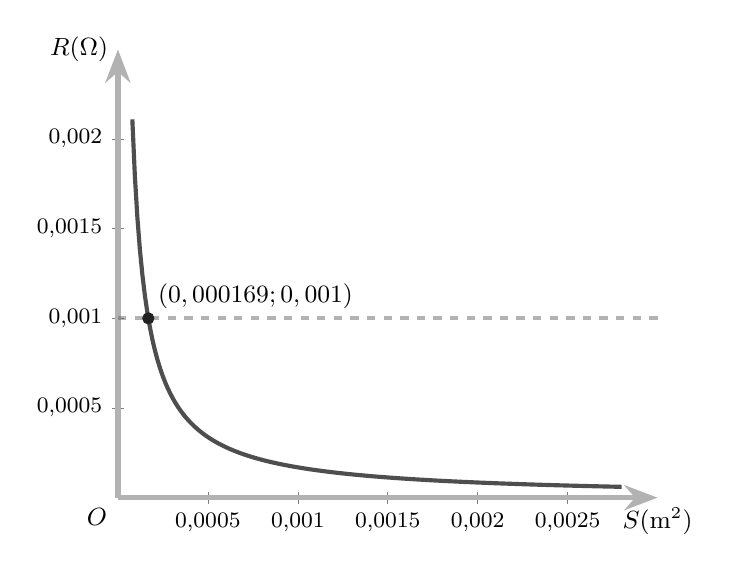
\begin{tikzpicture}
\begin{axis}[
    font=\small\sf,
    axis lines=middle,
    axis line style={->, line width=2pt, color=den-6!50},
    xlabel={$S (\mathrm{m}^2)$},
    ylabel={$R (\Omega)$},
    xlabel style={below, font=\small\sf},
    ylabel style={left, font=\small\sf},
    domain=0.00001:0.0028,  
    restrict y to domain=0:.0025,
    samples=200,
    ymin=0, ymax=.0025,
    xmin=0, xmax=0.003,
    ytick={0.0005, 0.001, 0.0015, 0.002},
    yticklabels={$0\mathrm{,}0005$, $0\mathrm{,}001$, $0\mathrm{,}0015$, $0\mathrm{,}002$},
    % xtick style={draw=none},
    xtick={0.0005, 0.001, 0.0015, 0.002, 0.0025},    
    xticklabels={$0\mathrm{,}0005$, $0\mathrm{,}001$, $0\mathrm{,}0015$, $0\mathrm{,}002$,$0\mathrm{,}0025$}, 
    % ytick style={draw=none},
    tick label style={font=\footnotesize},
    % tick label style={font=\footnotesize\sf, /pgf/number format/use comma, /pgf/number format/1000 sep={}},
    scaled ticks=false,
    % grid=major,
    clip=false,
  ]
    
\addplot[
      line width=1.5pt, 
      color=den-2, 
      opacity=.8
      ]
        {1.69e-8 * 10 / x};

\addplot[dashed, line width=1.5pt, color=den-6, opacity=.5] coordinates {
        (0,.001)
        (.003,.001)
        };

\addplot[only marks, mark=*, mark size=2pt, color=den-2] coordinates {
        (.000169,.001)
        };

\node[originlabel] at (axis cs:0,0) {$O$};
\node at (.000169,.001) [above right] {$(0,000169;0,001)$};

\end{axis}
\end{tikzpicture}

\end{document}
